\documentclass[landscape]{article}
\usepackage[a4paper, margin=1cm]{geometry}
\usepackage{tikz}
\usetikzlibrary{shapes,arrows,positioning,fit,backgrounds,calc,shadows}

\begin{document}

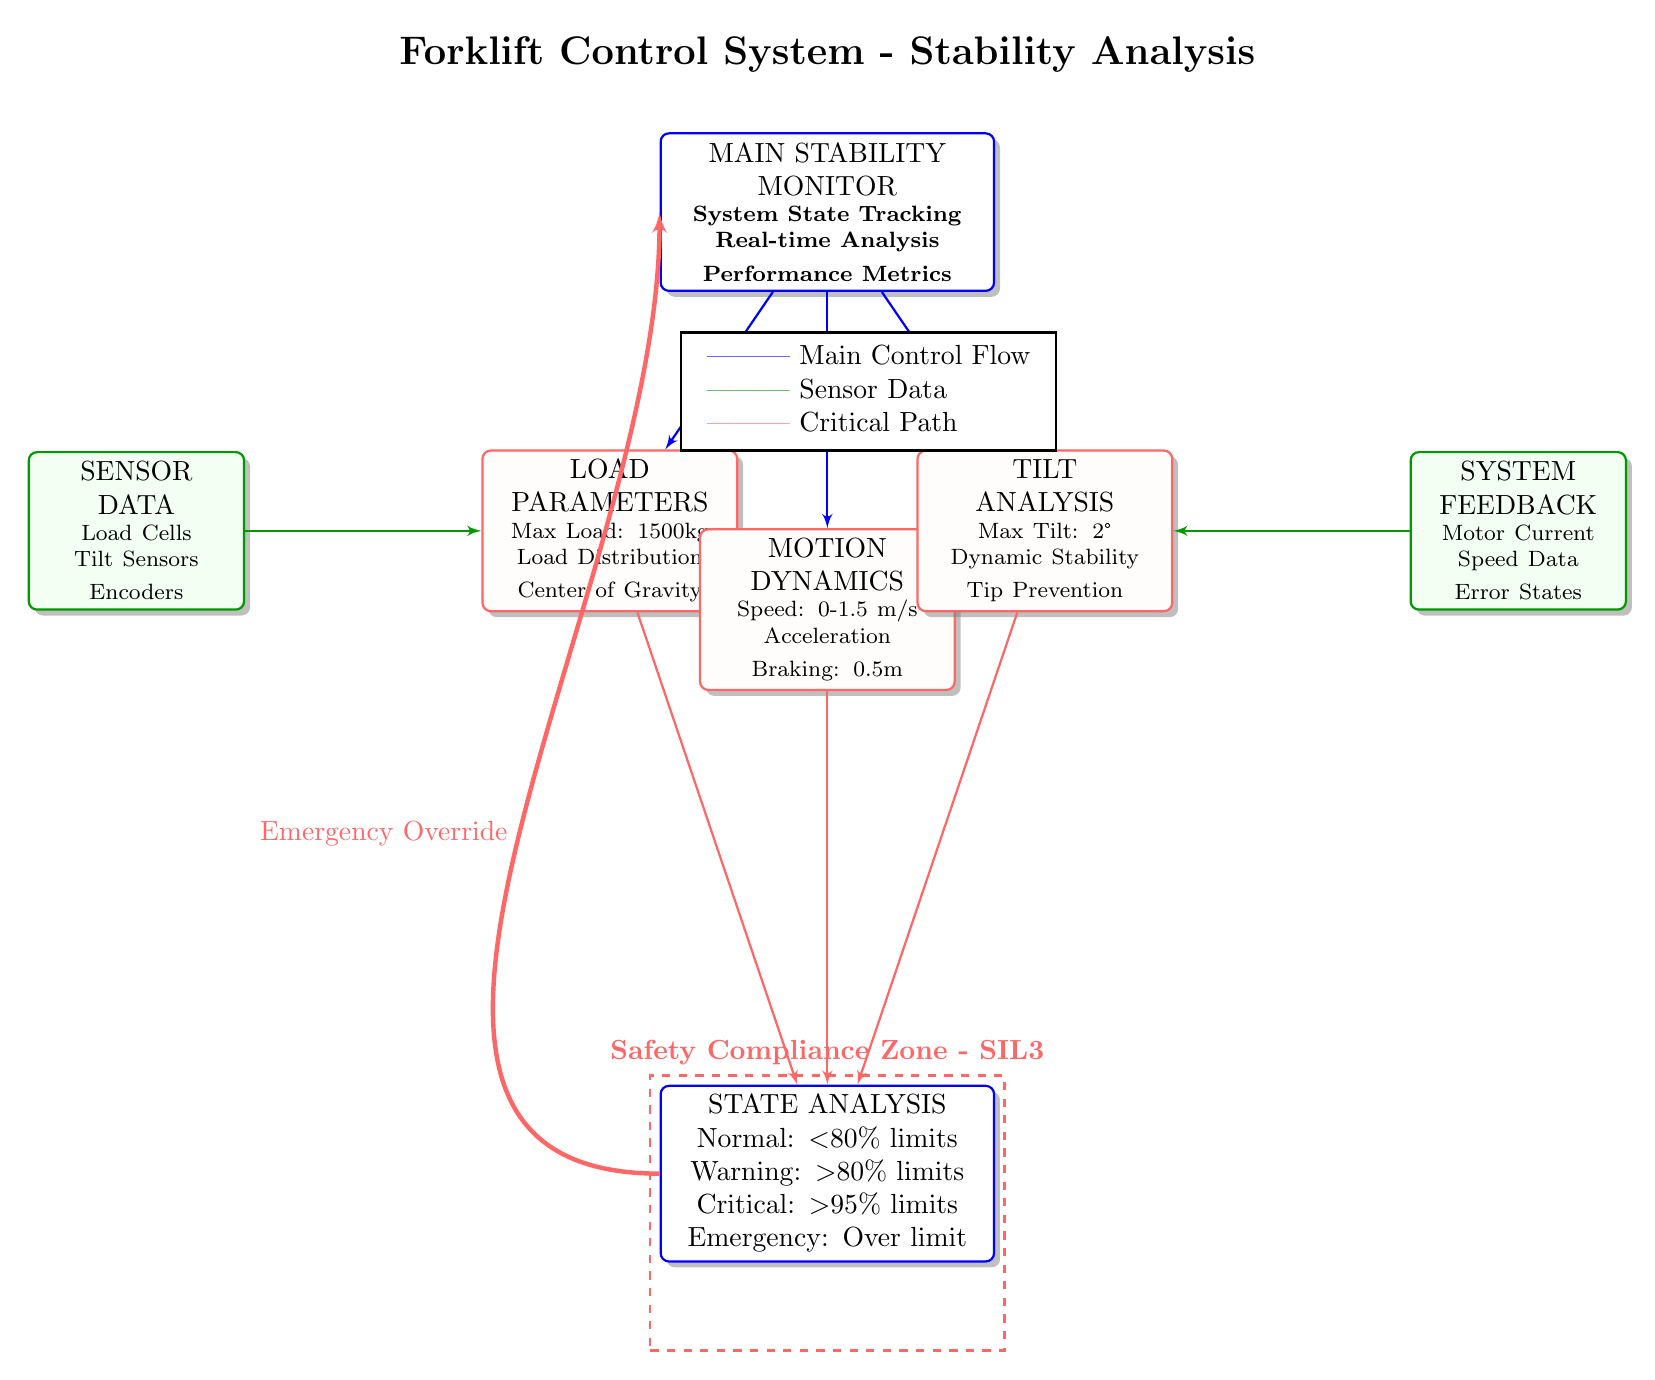
\begin{tikzpicture}[
    auto,
    mainblock/.style={
        rectangle,
        draw=blue,
        thick,
        text width=4cm,
        minimum height=2cm,
        align=center,
        rounded corners=3pt,
        fill=white,
        drop shadow
    },
    sensorblock/.style={
        rectangle,
        draw=green!60!black,
        thick,
        text width=2.5cm,
        minimum height=2cm,
        align=center,
        rounded corners=3pt,
        fill=green!5,
        drop shadow
    },
    paramblock/.style={
        rectangle,
        draw=red!60,
        thick,
        text width=3cm,
        minimum height=2cm,
        align=center,
        rounded corners=3pt,
        fill=pink!5,
        drop shadow
    },
    line/.style={draw=blue, thick, -latex'},
    sensor line/.style={draw=green!60!black, thick, -latex'},
    critical line/.style={draw=red!60, thick, -latex'}
]

% Title
\node [font=\Large\bfseries] at (0,4) {Forklift Control System - Stability Analysis};

% Main Stability Monitor
\node [mainblock] (monitor) at (0,2) {MAIN STABILITY\\MONITOR\\
    \footnotesize
    \textbf{System State Tracking}\\
    \textbf{Real-time Analysis}\\
    \textbf{Performance Metrics}};

% Parameter Blocks
\node [paramblock, below left=2cm and -1cm of monitor] (load) {LOAD\\PARAMETERS\\
    \footnotesize
    Max Load: 1500kg\\
    Load Distribution\\
    Center of Gravity};

\node [paramblock, below=3cm of monitor] (motion) {MOTION\\DYNAMICS\\
    \footnotesize
    Speed: 0-1.5 m/s\\
    Acceleration\\
    Braking: 0.5m};

\node [paramblock, below right=2cm and -1cm of monitor] (tilt) {TILT\\ANALYSIS\\
    \footnotesize
    Max Tilt: 2°\\
    Dynamic Stability\\
    Tip Prevention};

% Sensor and Feedback Blocks
\node [sensorblock, left=3cm of load] (sensors) {SENSOR\\DATA\\
    \footnotesize
    Load Cells\\
    Tilt Sensors\\
    Encoders};

\node [sensorblock, right=3cm of tilt] (feedback) {SYSTEM\\FEEDBACK\\
    \footnotesize
    Motor Current\\
    Speed Data\\
    Error States};

% State Analysis Block with proper LaTeX symbols
\node [mainblock, below=5cm of motion] (state) {STATE ANALYSIS\\
    Normal: {$<$}80\% limits\\
    Warning: {$>$}80\% limits\\
    Critical: {$>$}95\% limits\\
    Emergency: Over limit};


% Safety Box
\begin{scope}[on background layer]
    \node[draw=red!60, thick, dashed, fit={(state) ($(state.south)+(0,-1)$)}] 
        (safety_box) {};
    \node[above] at (safety_box.north) {\color{red!60}\textbf{Safety Compliance Zone - SIL3}};
\end{scope}

% Connections
\draw [line] (monitor) -- (load);
\draw [line] (monitor) -- (motion);
\draw [line] (monitor) -- (tilt);
\draw [sensor line] (sensors) -- (load);
\draw [sensor line] (feedback) -- (tilt);
\draw [critical line] (load) -- (state);
\draw [critical line] (motion) -- (state);
\draw [critical line] (tilt) -- (state);

% Emergency Override
\draw [critical line, ultra thick] (state.west) to [out=180, in=270] 
    node[left, text=red!60] {Emergency Override} 
    (monitor.west);

% Add legend
\node[draw, thick, fill=white, below right=0.5cm and -4cm of monitor] {
    \begin{tabular}{ll}
        \textcolor{blue}{―――} Main Control Flow\\
        \textcolor{green!60!black}{―――} Sensor Data\\
        \textcolor{red!60}{―――} Critical Path
    \end{tabular}
};

\end{tikzpicture}

\end{document} 